\begin{appendices}

%%%%%%%%%%%%%%%%%%%%%%%%%%%%%%%%%%%%%%%%%%%%%%%%%%%%%%%%%%%%%%%%%%%%%%%%%%%%%%%
\chapter{Energy Group Structures}
\label{app:energy-groups}

The energy group structures are from the CASMO-4 lattice physics code~\cite{edenius1995casmo}. The author gratefully acknowledges Geoffrey Gunow for his assistance in obtaining the structures.

\renewcommand{\arraystretch}{0.8}% Tighter

\begin{table}[h!]
  \centering
  \footnotesize
  \caption{One group structure.}
  \label{table:app-1-groups} 
  \vspace{14pt}
  \begin{tabular}{c r r}
    \toprule
    {\bf Group No.} &
    {\bf Lower Bound [MeV]} &
    {\bf Upper Bound [MeV]} \\
    \midrule
1 & 0.0000E+00 & 2.0000E+01 \\
    \bottomrule
   \end{tabular}
\end{table}

\begin{table}[h!]
  \centering
  \footnotesize
  \caption{Two group structure.}
  \label{table:app-2-groups} 
  \vspace{14pt}
  \begin{tabular}{c r r}
    \toprule
    {\bf Group No.} &
    {\bf Lower Bound [MeV]} &
    {\bf Upper Bound [MeV]} \\
    \midrule
2 & 0.0000E+00 & 6.2500E-07 \\
1 & 6.2500E-07 & 2.0000E+01 \\
  \bottomrule
 \end{tabular}
\end{table}

\begin{table}[h!]
  \centering
  \footnotesize
  \caption{Four group structure.}
  \label{table:app-4-groups} 
  \vspace{14pt}
  \begin{tabular}{c r r}
    \toprule
    {\bf Group No.} &
    {\bf Lower Bound [MeV]} &
    {\bf Upper Bound [MeV]} \\
    \midrule
4 & 0.0000E+00 & 6.2500E-07 \\
3 & 6.2500E-07 & 5.5300E-03 \\
2 & 5.5300E-03 & 8.2100E-01 \\
1 & 8.2100E-01 & 2.0000E+01 \\
  \bottomrule
 \end{tabular}
\end{table}

\begin{table}[h!]
  \centering
  \footnotesize
  \caption{Eight group structure.}
  \label{table:app-8-groups} 
  \vspace{14pt}
  \begin{tabular}{c r r}
    \toprule
    {\bf Group No.} &
    {\bf Lower Bound [MeV]} &
    {\bf Upper Bound [MeV]} \\
    \midrule
8 & 0.0000E+00 & 5.8000E-08 \\
7 & 5.8000E-08 & 1.4000E-07 \\
6 & 1.4000E-07 & 2.8000E-07 \\
5 & 2.8000E-07 & 6.2500E-07 \\
4 & 6.2500E-07 & 4.0000E-06 \\
3 & 4.0000E-06 & 5.5300E-03 \\
2 & 5.5300E-03 & 8.2100E-01 \\
1 & 8.2100E-01 & 2.0000E+01 \\
  \bottomrule
 \end{tabular}
\end{table}

\begin{table}[h!]
  \centering
  \footnotesize
  \caption{Sixteen group structure.}
  \label{table:app-16-groups} 
  \vspace{14pt}
  \begin{tabular}{c r r}
    \toprule
    {\bf Group No.} &
    {\bf Lower Bound [MeV]} &
    {\bf Upper Bound [MeV]} \\
    \midrule
16 & 0.0000E+00 & 3.0000E-08 \\
15 & 3.0000E-08 & 5.8000E-08 \\
14 & 5.8000E-08 & 1.4000E-07 \\
13 & 1.4000E-07 & 2.8000E-07 \\
12 & 2.8000E-07 & 3.5000E-07 \\
11 & 3.5000E-07 & 6.2500E-07 \\
10 & 6.2500E-07 & 8.5000E-07 \\
9 & 8.5000E-07 & 9.7200E-07 \\
8 & 9.7200E-07 & 1.0200E-06 \\
7 & 1.0200E-06 & 1.0970E-06 \\
6 & 1.0970E-06 & 1.1500E-06 \\
5 & 1.1500E-06 & 1.3000E-06 \\
4 & 1.3000E-06 & 4.0000E-06 \\
3 & 4.0000E-06 & 5.5300E-03 \\
2 & 5.5300E-03 & 8.2100E-01 \\
1 & 8.2100E-01 & 2.0000E+01 \\
  \bottomrule
 \end{tabular}
\end{table}

\begin{table}[h!]
  \centering
  \footnotesize
  \caption{Twenty-five group structure.}
  \label{table:app-25-groups} 
  \vspace{14pt}
  \begin{tabular}{c r r}
    \toprule
    {\bf Group No.} &
    {\bf Lower Bound [MeV]} &
    {\bf Upper Bound [MeV]} \\
    \midrule
25 & 0.0000E+00 & 3.0000E-08 \\
24 & 3.0000E-08 & 5.8000E-08 \\
23 & 5.8000E-08 & 1.4000E-07 \\
22 & 1.4000E-07 & 2.8000E-07 \\
21 & 2.8000E-07 & 3.5000E-07 \\
20 & 3.5000E-07 & 6.2500E-07 \\
19 & 6.2500E-07 & 9.7200E-07 \\
18 & 9.7200E-07 & 1.0200E-06 \\
17 & 1.0200E-06 & 1.0970E-06 \\
16 & 1.0970E-06 & 1.1500E-06 \\
15 & 1.1500E-06 & 1.8550E-06 \\
14 & 1.8550E-06 & 4.0000E-06 \\
13 & 4.0000E-06 & 9.8770E-06 \\
12 & 9.8770E-06 & 1.5968E-05 \\
11 & 1.5968E-05 & 1.4873E-04 \\
10 & 1.4873E-04 & 5.5300E-03 \\
9 & 5.5300E-03 & 9.1180E-03 \\
8 & 9.1180E-03 & 1.1100E-01 \\
7 & 1.1100E-01 & 5.0000E-01 \\
6 & 5.0000E-01 & 8.2100E-01 \\
5 & 8.2100E-01 & 1.3530E+00 \\
4 & 1.3530E+00 & 2.2310E+00 \\
3 & 2.2310E+00 & 3.6790E+00 \\
2 & 3.6790E+00 & 6.0655E+00 \\
1 & 6.0655E+00 & 2.0000E+01 \\
  \bottomrule
 \end{tabular}
\end{table}

\begin{table}[h!]
  \centering	
  \footnotesize
  \caption{Forty group structure.}
  \label{table:app-40-groups} 
  \vspace{14pt}
  \begin{tabular}{c r r}
    \toprule
    {\bf Group No.} &
    {\bf Lower Bound [MeV]} &
    {\bf Upper Bound [MeV]} \\
    \midrule
40 & 0.0000E+00 & 1.5000E-08 \\
39 & 1.5000E-08 & 3.0000E-08 \\
38 & 3.0000E-08 & 4.2000E-08 \\
37 & 4.2000E-08 & 5.8000E-08 \\
36 & 5.8000E-08 & 8.0000E-08 \\
35 & 8.0000E-08 & 1.0000E-07 \\
34 & 1.0000E-07 & 1.4000E-07 \\
33 & 1.4000E-07 & 1.8000E-07 \\
32 & 1.8000E-07 & 2.2000E-07 \\
31 & 2.2000E-07 & 2.8000E-07 \\
30 & 2.8000E-07 & 3.5000E-07 \\
29 & 3.5000E-07 & 6.2500E-07 \\
28 & 6.2500E-07 & 8.5000E-07 \\
27 & 8.5000E-07 & 9.5000E-07 \\
26 & 9.5000E-07 & 9.7200E-07 \\
25 & 9.7200E-07 & 1.0200E-06 \\
24 & 1.0200E-06 & 1.0970E-06 \\
23 & 1.0970E-06 & 1.1500E-06 \\
22 & 1.1500E-06 & 1.3000E-06 \\
21 & 1.3000E-06 & 1.5000E-06 \\
20 & 1.5000E-06 & 1.8550E-06 \\
19 & 1.8550E-06 & 2.1000E-06 \\
18 & 2.1000E-06 & 2.6000E-06 \\
17 & 2.6000E-06 & 3.3000E-06 \\
16 & 3.3000E-06 & 4.0000E-06 \\
15 & 4.0000E-06 & 9.8770E-06 \\
14 & 9.8770E-06 & 1.5968E-05 \\
13 & 1.5968E-05 & 2.7700E-05 \\
12 & 2.7700E-05 & 4.8052E-05 \\
11 & 4.8052E-05 & 1.4873E-04 \\
10 & 1.4873E-04 & 5.5300E-03 \\
9 & 5.5300E-03 & 9.1180E-03 \\
8 & 9.1180E-03 & 1.1100E-01 \\
7 & 1.1100E-01 & 5.0000E-01 \\
6 & 5.0000E-01 & 8.2100E-01 \\
5 & 8.2100E-01 & 1.3530E+00 \\
4 & 1.3530E+00 & 2.2310E+00 \\
3 & 2.2310E+00 & 3.6790E+00 \\
2 & 3.6790E+00 & 6.0655E+00 \\
1 & 6.0655E+00 & 2.0000E+01 \\
  \bottomrule
 \end{tabular}
\end{table}


\afterpage{
\renewcommand*{\arraystretch}{0.6}% Tighter
\footnotesize
\begin{longtable}[h!]{c r r}
  \caption{Seventy group structure.} \\
  \label{table:app-70-groups} \\
  \toprule
  {\bf Group No.} &
  {\bf Lower Bound [MeV]} &
  {\bf Upper Bound [MeV]} \\
  \midrule
70 & 0.0000E+00 & 5.0000E-09 \\
69 & 5.0000E-09 & 1.0000E-08 \\
68 & 1.0000E-08 & 1.5000E-08 \\
67 & 1.5000E-08 & 2.0000E-08 \\
66 & 2.0000E-08 & 2.5000E-08 \\
65 & 2.5000E-08 & 3.0000E-08 \\
64 & 3.0000E-08 & 3.5000E-08 \\
63 & 3.5000E-08 & 4.2000E-08 \\
62 & 4.2000E-08 & 5.0000E-08 \\
61 & 5.0000E-08 & 5.8000E-08 \\
60 & 5.8000E-08 & 6.7000E-08 \\
59 & 6.7000E-08 & 8.0000E-08 \\
58 & 8.0000E-08 & 1.0000E-07 \\
57 & 1.0000E-07 & 1.4000E-07 \\
56 & 1.4000E-07 & 1.8000E-07 \\
55 & 1.8000E-07 & 2.2000E-07 \\
54 & 2.2000E-07 & 2.5000E-07 \\
53 & 2.5000E-07 & 2.8000E-07 \\
52 & 2.8000E-07 & 3.0000E-07 \\
51 & 3.0000E-07 & 3.2000E-07 \\
50 & 3.2000E-07 & 3.5000E-07 \\
49 & 3.5000E-07 & 4.0000E-07 \\
48 & 4.0000E-07 & 5.0000E-07 \\
47 & 5.0000E-07 & 6.2500E-07 \\
46 & 6.2500E-07 & 7.8000E-07 \\
45 & 7.8000E-07 & 8.5000E-07 \\
44 & 8.5000E-07 & 9.1000E-07 \\
43 & 9.1000E-07 & 9.5000E-07 \\
42 & 9.5000E-07 & 9.7200E-07 \\
41 & 9.7200E-07 & 9.9600E-07 \\
40 & 9.9600E-07 & 1.0200E-06 \\
39 & 1.0200E-06 & 1.0450E-06 \\
38 & 1.0450E-06 & 1.0710E-06 \\
37 & 1.0710E-06 & 1.0970E-06 \\
36 & 1.0970E-06 & 1.1230E-06 \\
35 & 1.1230E-06 & 1.1500E-06 \\
34 & 1.1500E-06 & 1.3000E-06 \\
33 & 1.3000E-06 & 1.5000E-06 \\
32 & 1.5000E-06 & 1.8550E-06 \\
31 & 1.8550E-06 & 2.1000E-06 \\
30 & 2.1000E-06 & 2.6000E-06 \\
29 & 2.6000E-06 & 3.3000E-06 \\
28 & 3.3000E-06 & 4.0000E-06 \\
27 & 4.0000E-06 & 9.8770E-06 \\
26 & 9.8770E-06 & 1.5968E-05 \\
25 & 1.5968E-05 & 2.7700E-05 \\
24 & 2.7700E-05 & 4.8052E-05 \\
23 & 4.8052E-05 & 7.5501E-05 \\
22 & 7.5501E-05 & 1.4873E-04 \\
21 & 1.4873E-04 & 3.6726E-04 \\
20 & 3.6726E-04 & 9.0690E-04 \\
19 & 9.0690E-04 & 1.4251E-03 \\
18 & 1.4251E-03 & 2.2395E-03 \\
17 & 2.2395E-03 & 3.5191E-03 \\
16 & 3.5191E-03 & 5.5300E-03 \\
15 & 5.5300E-03 & 9.1180E-03 \\
14 & 9.1180E-03 & 1.5030E-02 \\
13 & 1.5030E-02 & 2.4780E-02 \\
12 & 2.4780E-02 & 4.0850E-02 \\
11 & 4.0850E-02 & 6.7340E-02 \\
10 & 6.7340E-02 & 1.1100E-01 \\
9 & 1.1100E-01 & 1.8300E-01 \\
8 & 1.8300E-01 & 3.0250E-01 \\
7 & 3.0250E-01 & 5.0000E-01 \\
6 & 5.0000E-01 & 8.2100E-01 \\
5 & 8.2100E-01 & 1.3530E+00 \\
4 & 1.3530E+00 & 2.2310E+00 \\
3 & 2.2310E+00 & 3.6790E+00 \\
2 & 3.6790E+00 & 6.0655E+00 \\
1 & 6.0655E+00 & 2.0000E+01 \\
  \bottomrule
\end{longtable}}


%%%%%%%%%%%%%%%%%%%%%%%%%%%%%%%%%%%%%%%%%%%%%%%%%%%%%%%%%%%%%%%%%%%%%%%%%%%%%%%
\chapter{Heterogeneous BEAVRS Model Parameters}
\label{app:beavrs-benchmarks}

%%%%%%%%%%%%%%%%%%%%%%%%%%%%%%%%%%%%%%%%
\section{Material Isotopic Compositions}
\label{sec:beavrs-materials}

The isotopic compositions used in the \ac{PWR} benchmark models in Part IV were identical to those in the \ac{BEAVRS} \ac{PWR} model v1.1.1~\cite{horelik2013beavrs} and are reproduced in the tables below.

\begin{table}[h!]
  \centering
  \caption[BEAVRS isotopic composition for air]{Composition of air (0.000616 g/cc).}
  \footnotesize
  \label{table:chap7-beavrs-isotopes-air}
  \vspace{6pt}
  \begin{tabular}{c c}
  \toprule
  \rowcolor{lightgray}
  {\bf Nuclide} &
  {\bf Density [atom/b-cm]} \\
  \midrule
  C-12 & 6.7565e-09 \\
  C-13 & 7.3076e-11 \\
  O-16 & 5.2864e-06 \\
  O-17 & 2.0137e-09 \\
  N-14 & 1.9681e-05 \\
  N-15 & 7.1900e-08 \\
  Ar-36 & 7.9414e-10 \\
  Ar-38 & 1.4915e-10 \\
  Ar-40 & 2.3506e-07 \\
  \bottomrule
\end{tabular}
\end{table}

\begin{table}[h!]
  \centering
  \caption[BEAVRS isotopic composition for borated water]{Composition of borated water (0.740582 g/cc).}
  \footnotesize
  \label{table:chap7-beavrs-isotopes-water}
  \vspace{6pt}
  \begin{tabular}{c c}
  \toprule
  \rowcolor{lightgray}
  {\bf Nuclide} &
  {\bf Density [atom/b-cm]} \\
  \midrule
  H-1 & 4.9457e-02 \\
  H-2 & 7.4196e-06 \\
  B-10 & 8.0042e-06 \\
  B-11 & 3.2218e-05 \\
  O-16 & 2.4672e-02 \\
  O-17 & 9.3982e-06 \\
  \bottomrule
\end{tabular}
\end{table}

\begin{table}[h!]
  \centering
  \caption[BEAVRS isotopic composition for borosilicate glass]{Composition of borosilicate glass (2.260000 g/cc).}
  \footnotesize
  \label{table:chap7-beavrs-isotopes-borosilicate}
  \vspace{6pt}
  \begin{tabular}{c c}
  \toprule
  \rowcolor{lightgray}
  {\bf Nuclide} &
  {\bf Density [atom/b-cm]} \\
  \midrule
  B-10 & 9.6506e-04 \\
  B-11 & 3.9189e-03 \\
  O-16 & 4.6511e-02 \\
  O-17 & 1.7717e-05 \\
  Al-27 & 1.7352e-03 \\
  Si-28 & 1.6924e-02 \\
  Si-29 & 8.5977e-04 \\
  Si-30 & 5.6743e-04 \\
  \bottomrule
\end{tabular}
\end{table}

\begin{table}[h!]
  \centering
  \caption[BEAVRS isotopic composition for 1.6\% enriched UO$_2$]{Composition of 1.6\% enriched UO$_2$ fuel (10.31341 g/cc).}
  \footnotesize
  \label{table:chap7-beavrs-isotopes-1.6-uo2}
  \vspace{6pt}
  \begin{tabular}{c c}
  \toprule
  \rowcolor{lightgray}
  {\bf Nuclide} &
  {\bf Density [atom/b-cm]} \\
  \midrule
  U-234 & 3.0131E-06 \\
  U-235 & 3.7503E-04 \\
  U-238 & 2.2625e-02 \\
  O-16 & 4.5895e-02 \\
  O-17 & 1.7482e-05 \\
  \bottomrule
\end{tabular}
\end{table}

\begin{table}[h!]
  \centering
  \caption[BEAVRS isotopic composition for 3.1\% enriched UO$_2$]{Composition of 3.1\% enriched UO$_2$ fuel (10.34115 g/cc).}
  \footnotesize
  \label{table:chap7-beavrs-isotopes-3.1-uo2}
  \vspace{6pt}
  \begin{tabular}{c c}
  \toprule
  \rowcolor{lightgray}
  {\bf Nuclide} &
  {\bf Density [atom/b-cm]} \\
  \midrule
  U-234 & 5.7987e-06 \\
  U-235 & 7.2175e-04 \\
  U-238 & 2.2253e-02 \\
  O-16 & 4.5850e-02 \\
  O-17 & 1.7466e-05 \\
  \bottomrule
\end{tabular}
\end{table}

\begin{table}[h!]
  \centering
  \caption[BEAVRS isotopic composition for helium]{Composition of helium (0.001598 g/cc).}
  \footnotesize
  \label{table:chap7-beavrs-isotopes-3.1-helium}
  \vspace{6pt}
  \begin{tabular}{c c}
  \toprule
  \rowcolor{lightgray}
  {\bf Nuclide} &
  {\bf Density [atom/b-cm]} \\
  \midrule
  He-4 & 2.4044e-04 \\
  \bottomrule
\end{tabular}
\end{table}

\begin{table}[h!]
  \centering
  \caption[BEAVRS isotopic composition for stainless steel]{Composition of SS304 stainless steel (8.03 g/cc).}
  \footnotesize
  \label{table:chap7-beavrs-isotopes-3.1-stainless-steel}
  \vspace{6pt}
  \begin{tabular}{c c}
  \toprule
  \rowcolor{lightgray}
  {\bf Nuclide} &
  {\bf Density [atom/b-cm]} \\
  \midrule
  Si-28 & 9.5274e-04 \\
  Si-29 & 4.8400e-05 \\
  Si-30 & 3.1943e-05 \\
  Cr-50 & 7.6778e-04 \\
  Cr-52 & 1.4806e-02 \\
  Cr-53 & 1.6789e-03 \\
  Cr-54 & 4.1791e-04 \\
  Mn-55 & 1.7604e-03 \\
  Fe-54 & 3.4620e-03 \\
  Fe-56 & 5.4345e-02 \\
  Fe-57 & 1.2551e-03 \\
  Fe-58 & 1.6703e-04 \\
  Ni-58 & 5.6089e-03 \\
  Ni-60 & 2.1605e-03 \\
  Ni-61 & 9.3917e-05 \\
  Ni-62 & 2.9945e-04 \\
  Ni-64 & 7.6261e-05 \\
  \bottomrule
\end{tabular}
\end{table}

\begin{table}[h!]
  \centering
  \caption[BEAVRS isotopic composition for zircaloy]{Composition of zircaloy 4 (6.55 g/cc).}
  \footnotesize
  \label{table:chap7-beavrs-isotopes-3.1-zircaloy}
  \vspace{6pt}
  \begin{tabular}{c c}
  \toprule
  \rowcolor{lightgray}
  {\bf Nuclide} &
  {\bf Density [atom/b-cm]} \\
  \midrule
  O-16 & 3.0743e-04 \\
  O-17 & 1.1711e-07 \\
  Cr-50 & 3.2962e-06 \\
  Cr-52 & 6.3564e-05 \\
  Cr-53 & 7.2076e-06 \\
  Cr-54 & 1.7941e-06 \\
  Fe-54 & 8.6699e-06 \\
  Fe-56 & 1.3610e-04 \\
  Fe-57 & 3.1431e-06 \\
  Fe-58 & 4.1829e-07 \\
  Zr-90 & 2.1827e-02 \\
  Zr-91 & 4.7600e-03 \\
  Zr-92 & 7.2758e-03 \\
  Zr-94 & 7.3734e-03 \\
  Zr-96 & 1.1879e-03 \\
  Sn-112 & 4.6735e-06 \\
  Sn-114 & 3.1799e-06 \\
  Sn-115 & 1.6381e-06 \\
  Sn-116 & 7.0055e-05 \\
  Sn-117 & 3.7003e-05 \\
  Sn-118 & 1.1669e-04 \\
  Sn-119 & 4.1387e-05 \\
  Sn-120 & 1.5697e-04 \\
  Sn-122 & 2.2308e-05 \\
  Sn-124 & 2.7897e-05 \\
  \bottomrule
\end{tabular}
\end{table}

\clearpage

%%%%%%%%%%%%%%%%%%%%%%%%%%%%%%%%%%%%%%%%
\section{Geometric Configuration}
\label{sec:beavrs-geometry}

The geometric pin cell parameters for the \ac{PWR} benchmark models in Part IV were identical to those in the \ac{BEAVRS} \ac{PWR} model v1.1.1~\cite{horelik2013beavrs} at the core axial mid-plane. The pin cell radii are reproduced in the table below for clarity.

\renewcommand{\arraystretch}{0.9}
\begin{table}[h!]
  \centering
  \caption[BEAVRS pin cell radii]{Pin cell radii for the \ac{BEAVRS} model.}
  \small
  \label{table:app-pin-cell-radii} 
  \vspace{6pt}
  \begin{tabular}{l c}
  \toprule
  \rowcolor{lightgray}
  \multicolumn{1}{c}{\bf Material} &
  \multicolumn{1}{c}{\bf Radius [cm]} \\
  \midrule
  \multicolumn{2}{c}{\bf Fuel Pin} \\
  \midrule
  Fuel &  0.39218 \\
  Helium & 0.40005 \\
  Zircaloy & 0.45720 \\
  \midrule
  \multicolumn{2}{c}{\bf Control Rod Guide Tube} \\
  \midrule
  Borated Water & 0.56134 \\
  Zircaloy & 0.60198 \\
  \midrule
  \multicolumn{2}{c}{\bf Instrument Tube} \\
  \midrule
  Air & 0.43688 \\
  Zircaloy & 0.48387 \\
  Borated Water & 0.56134 \\
  Zircaloy & 0.60198 \\
  \midrule
  \multicolumn{2}{c}{\bf Burnable Poison} \\
  \midrule
  Air & 0.21400 \\
  Stainless Steel & 0.23051 \\
  Air & 0.24130 \\
  Borosilicate Glass & 0.42672 \\
  Air & 0.43688 \\
  Stainless Steel & 0.48387 \\
  Borated Water & 0.56134 \\
  Zircaloy & 0.60198 \\
  \bottomrule
\end{tabular}
\end{table}


%%%%%%%%%%%%%%%%%%%%%%%%%%%%%%%%%%%%%%%%
\section{BEAVRS Reaction Rates}
\label{sec:beavrs-rxn-rates}

The \ac{BEAVRS} reference reaction rate distributions used in Chap.~\ref{sec:chap7-motivate} were computed using isotropic in lab scattering in OpenMC to enable comparisons between OpenMC and OpenMOC. The fission and U-238 capture rate spatial distributions are highly skewed with this approximation. In particular, the distributions are significantly more peaked in assemblies the corner reflectors since the preferential streaming and leakage of neutrons through the reflector due to anisotropic scattering in water is not modeled. The ``true'' fission and U-238 capture rate spatial distributions computed using normal anisotropic scattering in OpenMC are illustrated below for comparison purpose, and as a reminder of the necessity for accurate models of higher order scattering in high-fidelity whole-core deterministic transport calculations.

\begin{figure}[h!]
\begin{subfigure}{\textwidth}
  \centering
  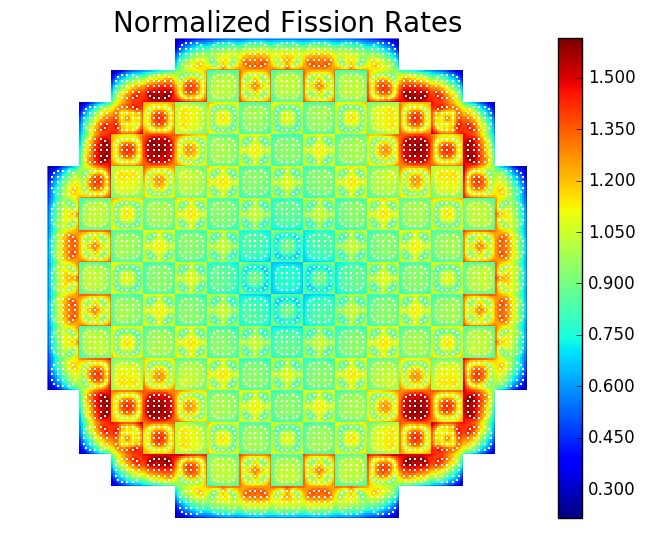
\includegraphics[width=0.75\linewidth]{figures/benchmarks/fission-rates/fiss-mean-full-core-aniso}
  \caption{}
  \label{fig:benchmarks-beavrs-fiss-aniso}
\end{subfigure}
\begin{subfigure}{\textwidth}
  \centering
  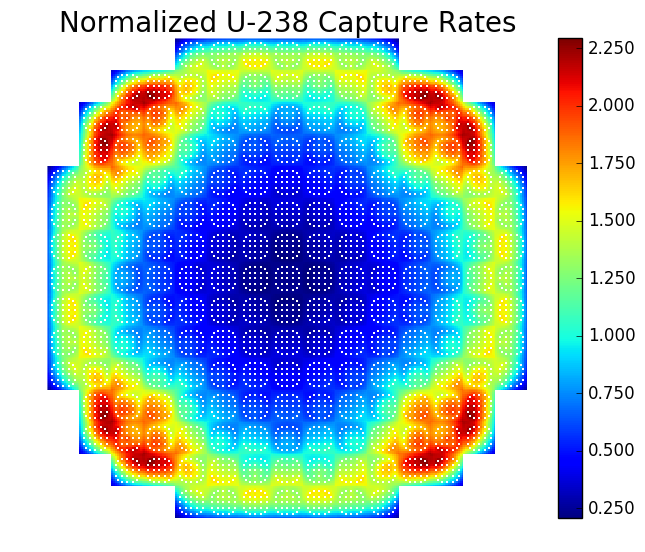
\includegraphics[width=0.75\linewidth]{figures/benchmarks/capture-rates/capt-mean-full-core-aniso}
  \caption{}
  \label{fig:benchmarks-beavrs-capt-aniso}
\end{subfigure}
\vspace{2mm}
\caption[BEAVRS pin-wise reaction rates from OpenMC with anisotropic scattering]{Fission rates (a) and U-238 capture rates (b) for the 2D quarter core \ac{BEAVRS} model tallied using a pin-wise mesh in OpenMC with anisotropic scattering.}
\label{fig:benchmarks-beavrs-aniso}
\end{figure}
	

%%%%%%%%%%%%%%%%%%%%%%%%%%%%%%%%%%%%%%%%%%%%%%%%%%%%%%%%%%%%%%%%%%%%%%%%%%%%%%%
\chapter{Quantification of Spatial Self-Shielding Effects}
\label{app:quantify-mgxs-shielding}

This section provides figures illustrating the impacts of the infinite, null and spatial homogenization as an addendum to Chap.~\ref{chap:quantify}. The percent relative fission and U-238 capture rate errors between OpenMC and OpenMOC for each homogenization scheme and benchmark for 2, 8 and 70 energy groups are illustrated in Sec.~\ref{sec:quantify-fiss-rates} and Sec.~\ref{sec:quantify-capt-rates}, respectively. Sec.~\ref{sec:quantify-capt-rates-absolute} illustrates the U-238 capture rate absolute errors for benchmarks with vacuum \acp{BC}.

%%%%%%%%%%%%%%%%%%%%%%%%%%%%%%%%%%%%%%
\section{Fission Rate Relative Errors}
\label{sec:quantify-fiss-rates}

The percent relative fission rate errors between OpenMC and OpenMOC for each homogenization scheme and benchmark for 2, 8 and 70 energy groups are shown in the following figures. These heatmaps complement Figs.~\Crefrange{fig:chap8-assm-1.6-fiss-err}{fig:chap8-full-core-fiss-err} by illustrating the error distributions for solutions computed by OpenMOC with 2-group \ac{MGXS}.

\begin{figure}[h!]
\centering
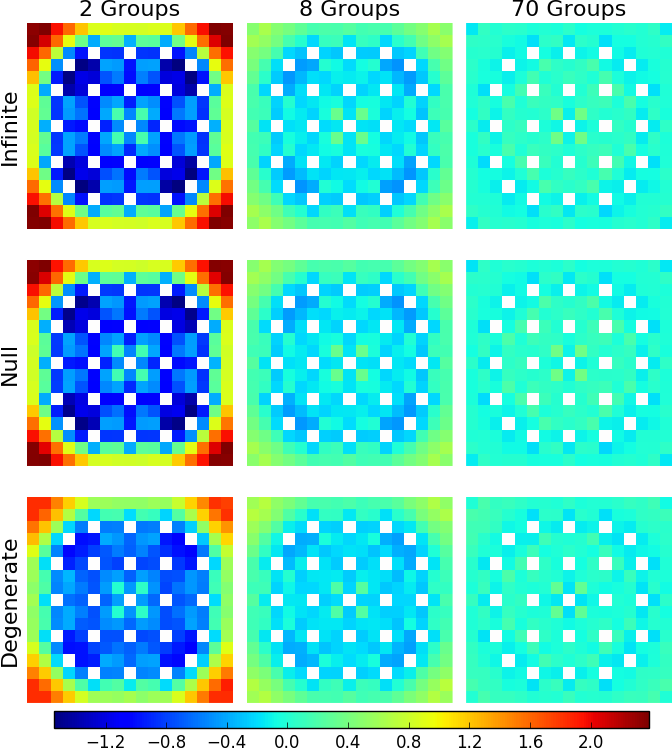
\includegraphics[width=\linewidth]{figures/quantification/appendix/assm-16/fiss-err}
\vspace{2mm}
\caption[Fission rate errors for a 1.6\% enriched assembly]{Fission rate percent relative errors for a 1.6\% enriched assembly corresponding to the reference in Fig.~\ref{fig:chap7-fiss-rates-1.6-assm}.}
\label{fig:quantify-assm-1.6-fiss-err}
\end{figure}

\clearpage

\begin{figure}[h!]
\centering
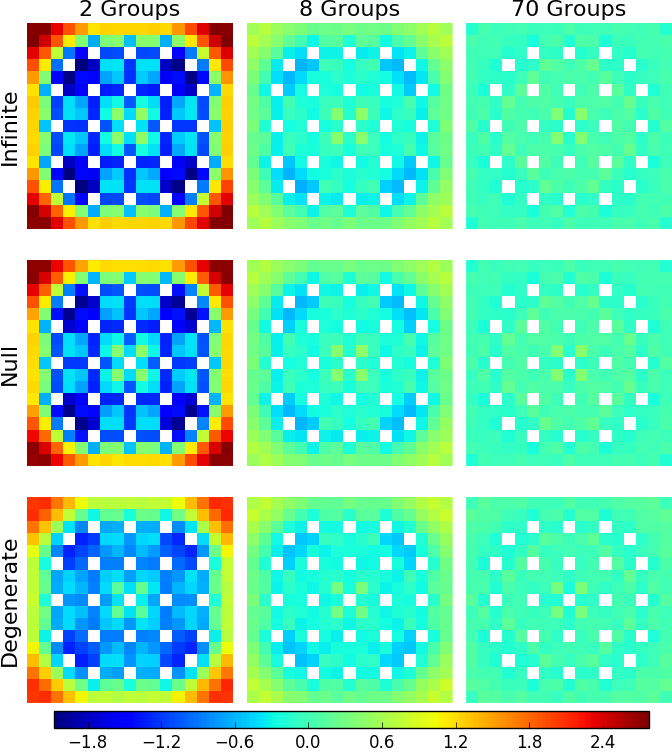
\includegraphics[width=\linewidth]{figures/quantification/appendix/assm-31/fiss-err}
\vspace{2mm}
\caption[Fission rate errors for a 3.1\% enriched assembly]{Fission rate percent relative errors for a 3.1\% enriched assembly corresponding to the reference in Fig.~\ref{fig:chap7-fiss-rates-3.1-assm}.}
\label{fig:quantify-assm-3.1-fiss-err}
\end{figure}

\clearpage

\begin{figure}[h!]
\centering
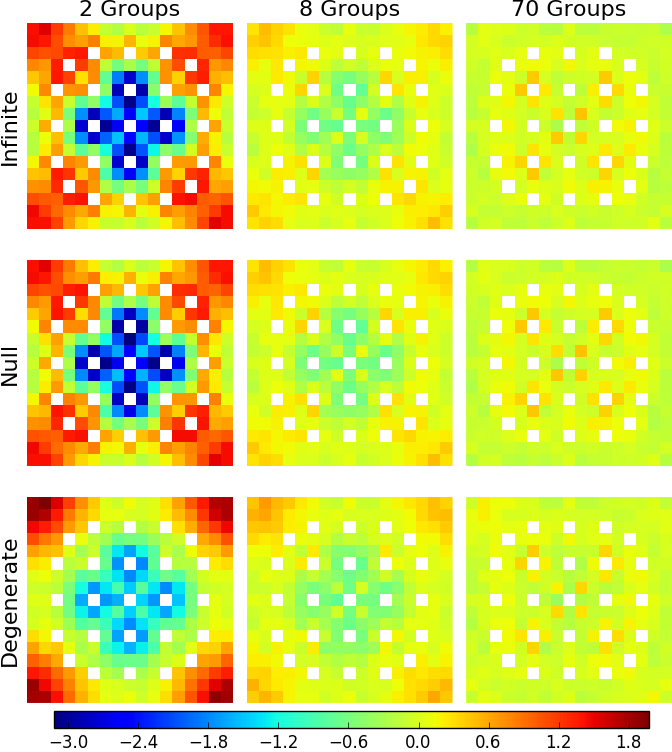
\includegraphics[width=\linewidth]{figures/quantification/appendix/assm-31-20BPs/fiss-err}
\vspace{2mm}
\caption[Fission rate errors for a 3.1\% enriched assembly with 20 BPs]{Fission rate percent relative errors for a 3.1\% enriched assembly with 20 BPs corresponding to the reference in Fig.~\ref{fig:chap7-fiss-rates-3.1-assm-20BAs}.}
\label{fig:quantify-assm-3.1-20BPs-fiss-err}
\end{figure}

\clearpage

\begin{figure}[h!]
\centering
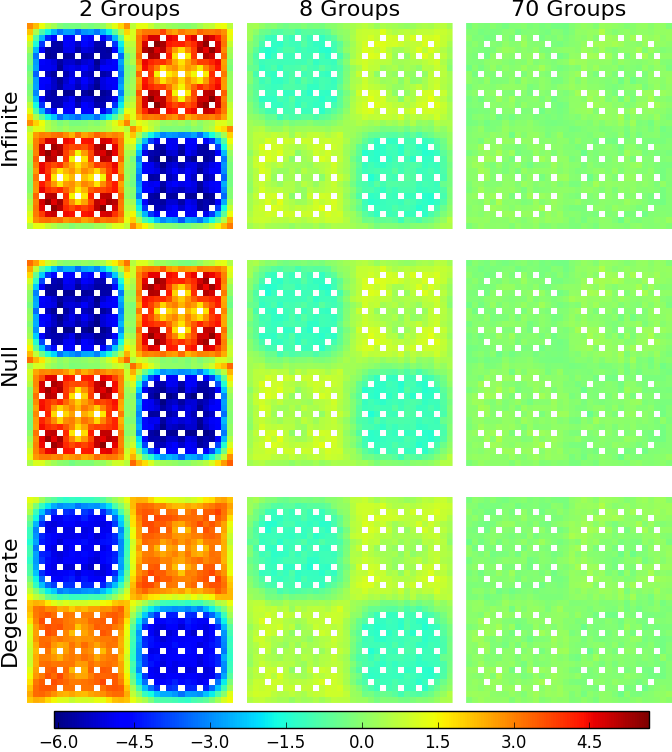
\includegraphics[width=\linewidth]{figures/quantification/appendix/2x2/fiss-err}
\vspace{2mm}
\caption[Fission rate errors for a 2$\times$2 colorset]{Fission rate percent relative errors for a 2$\times$2 colorset corresponding to the reference in Fig.~\ref{fig:chap7-fiss-rates-2x2}.}
\label{fig:quantify-2x2-fiss-err}
\end{figure}

\clearpage

\begin{figure}[h!]
\centering
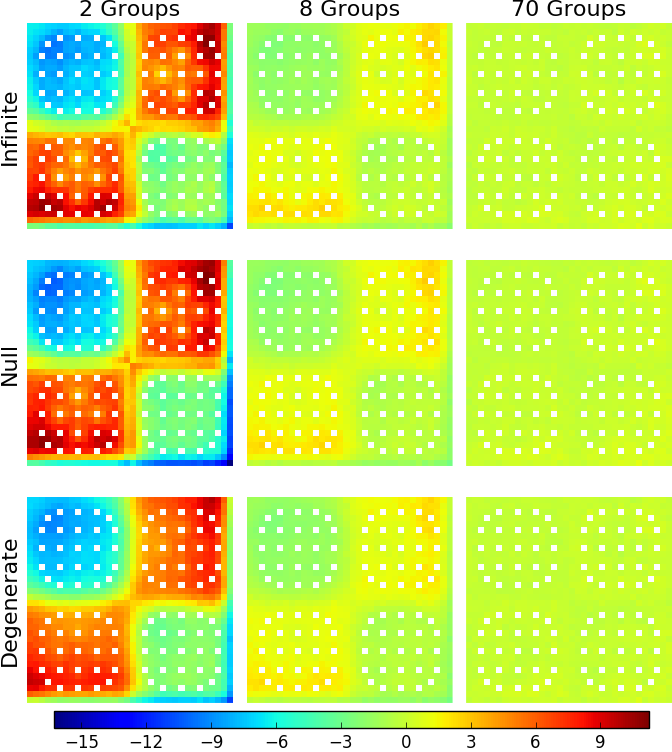
\includegraphics[width=\linewidth]{figures/quantification/appendix/reflector/fiss-err}
\vspace{2mm}
\caption[Fission rate errors for a 2$\times$2 colorset with a reflector]{Fission rate percent relative errors for a 2$\times$2 colorset with a reflector corresponding to the reference in Fig.~\ref{fig:chap7-fiss-rates-reflector}.}
\label{fig:quantify-reflector-fiss-err}
\end{figure}

\clearpage

\begin{figure}[h!]
\centering
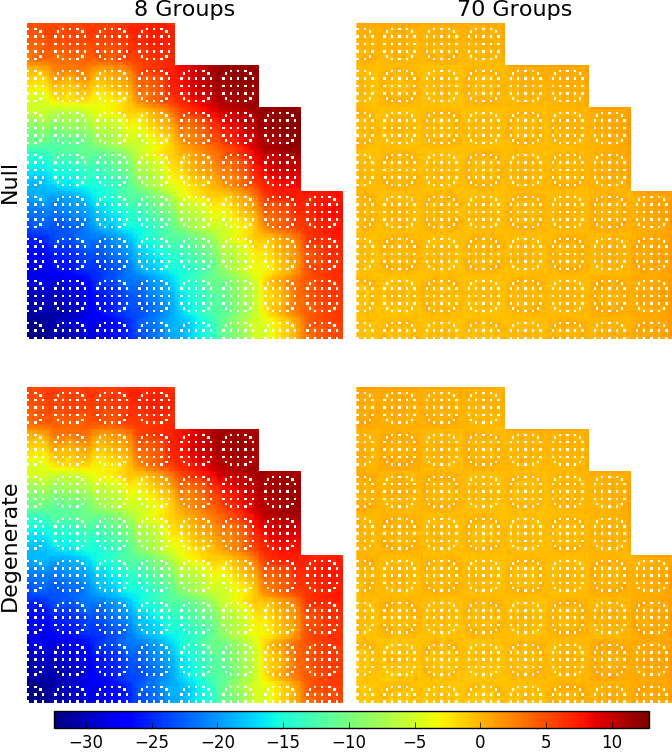
\includegraphics[width=\linewidth]{figures/quantification/appendix/full-core/fiss-err}
\vspace{2mm}
\caption[Fission rate errors for the 2D quarter core \ac{BEAVRS} model]{Fission rate percent relative errors for the quarter core \ac{BEAVRS} model corresponding to the reference in Fig.~\ref{fig:chap7-fiss-rates-full-core}.}
\label{fig:quantify-full-core-fiss-err}
\end{figure}

\clearpage


%%%%%%%%%%%%%%%%%%%%%%%%%%%%%%%%%%%%%%%%%%%%
\section{U-238 Capture Rate Relative Errors}
\label{sec:quantify-capt-rates}

The percent relative U-238 capture rate errors between OpenMC and OpenMOC for each spatial homogenization scheme and benchmark for 2, 8 and 70 energy groups are shown in the following figures. These heatmaps complement Figs.~\Crefrange{fig:chap8-assm-1.6-capt-err}{fig:chap8-full-core-capt-err} by illustrating the error distributions for solutions computed by OpenMOC with 2-group \ac{MGXS}.

\begin{figure}[h!]
\centering
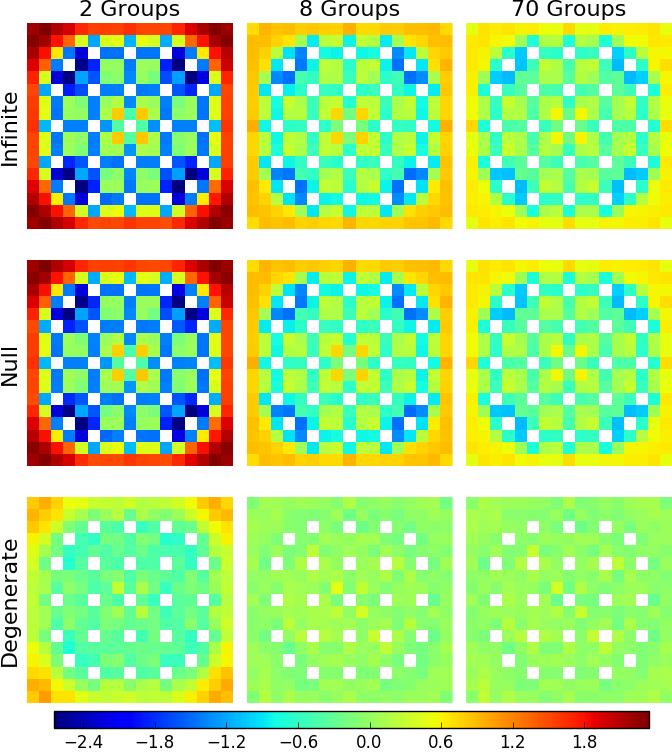
\includegraphics[width=\linewidth]{figures/quantification/appendix/assm-16/capt-err}
\vspace{2mm}
\caption[U-238 capture rate errors for a 1.6\% enriched assembly]{U-238 capture rate percent relative errors errors for a 1.6\% enriched assembly corresponding to the reference in Fig.~\ref{fig:chap7-capt-rates-1.6-assm}.}
\label{fig:quantify-assm-1.6-capt-err}
\end{figure}

\clearpage

\begin{figure}[h!]
\centering
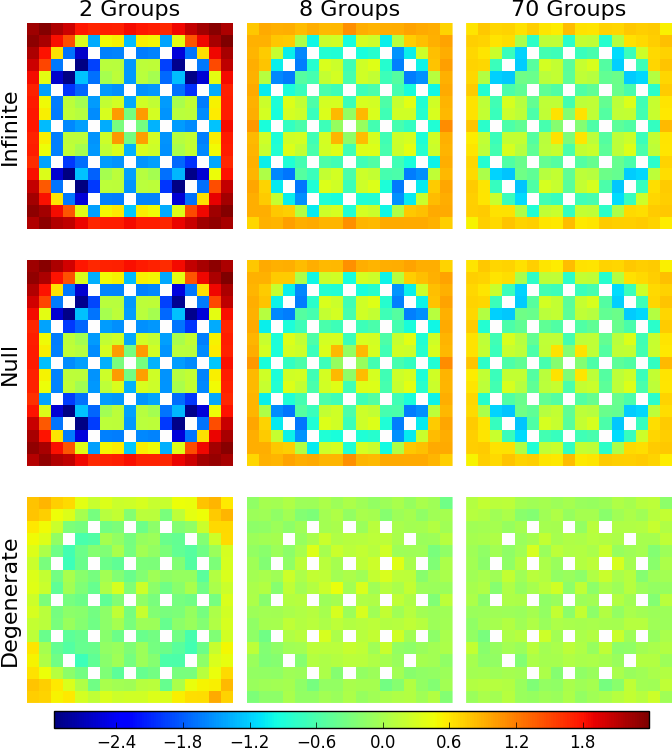
\includegraphics[width=\linewidth]{figures/quantification/appendix/assm-31/capt-err}
\vspace{2mm}
\caption[U-238 capture rate errors for a 3.1\% enriched assembly]{U-238 capture rate percent relative errors errors for a 3.1\% enriched assembly corresponding to the reference in Fig.~\ref{fig:chap7-capt-rates-3.1-assm}.}
\label{fig:quantify-assm-3.1-capt-err}
\end{figure}

\clearpage

\begin{figure}[h!]
\centering
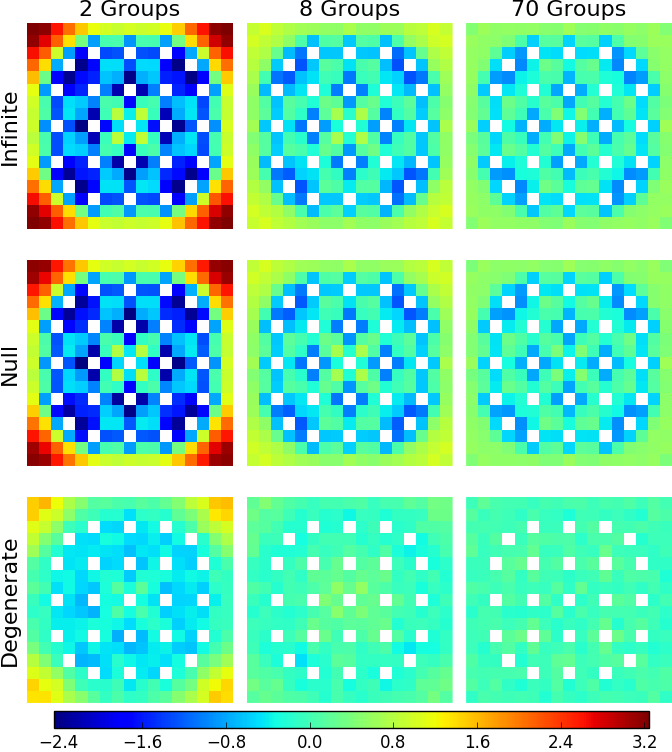
\includegraphics[width=\linewidth]{figures/quantification/appendix/assm-31-20BPs/capt-err}
\vspace{2mm}
\caption[U-238 capture rate errors for a 3.1\% enriched assembly with 20 BPs]{U-238 capture rate percent relative errors errors for a 3.1\% enriched assembly with 20 \acp{BP} corresponding to the reference in Fig.~\ref{fig:chap7-capt-rates-3.1-assm-20BAs}.}
\label{fig:quantify-assm-3.1-20BPs-capt-err}
\end{figure}

\clearpage

\begin{figure}[h!]
\centering
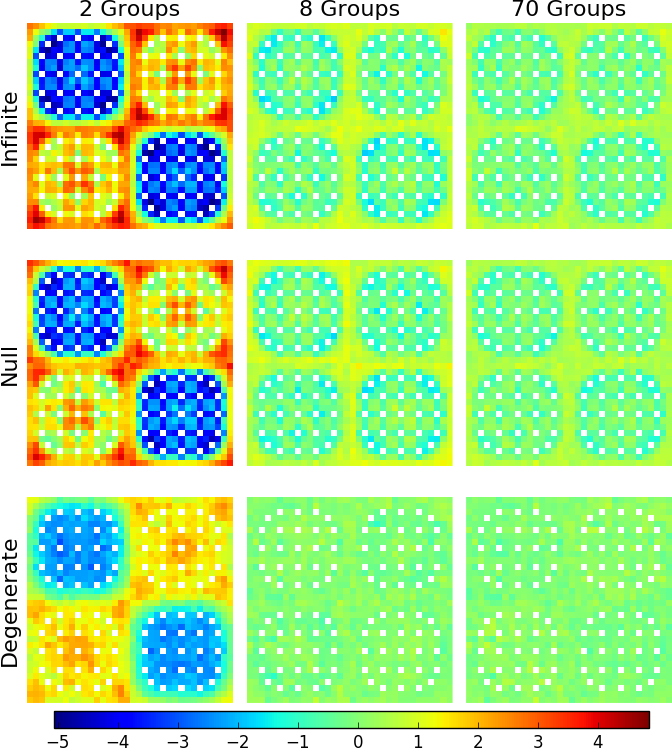
\includegraphics[width=\linewidth]{figures/quantification/appendix/2x2/capt-err}
\vspace{2mm}
\caption[U-238 capture rate errors for a 2$\times$2 colorset]{U-238 capture rate percent relative errors errors for a 2$\times$2 colorset corresponding to the reference in Fig.~\ref{fig:chap7-capt-rates-2x2}.}
\label{fig:quantify-2x2-capt-err}
\end{figure}

\clearpage

\begin{figure}[h!]
\centering
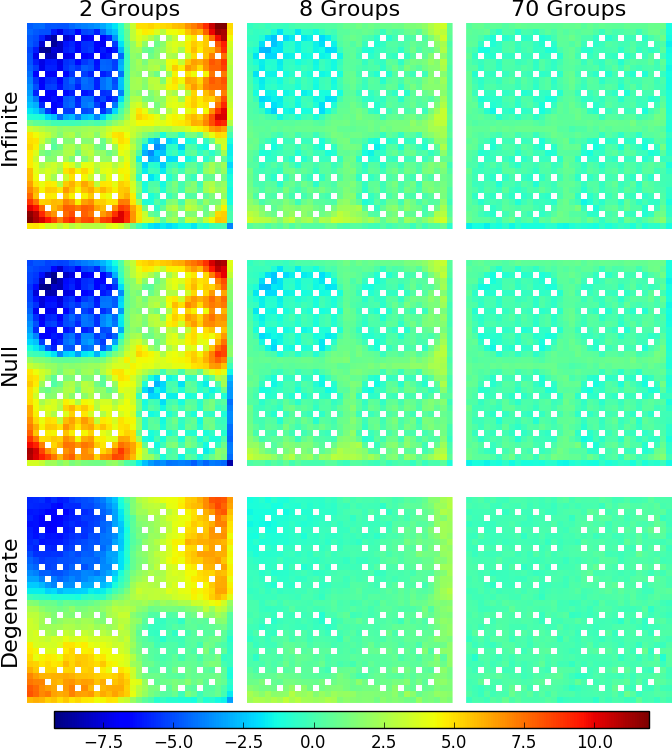
\includegraphics[width=\linewidth]{figures/quantification/appendix/reflector/capt-err}
\vspace{2mm}
\caption[U-238 capture rate errors for a 2$\times$2 colorset with a reflector]{U-238 capture percent relative errors rate errors for a 2$\times$2 colorset with a reflector corresponding to the reference in Fig.~\ref{fig:chap7-capt-rates-reflector}.}
\label{fig:quantify-reflector-capt-err}
\end{figure}

\clearpage

\begin{figure}[h!]
\centering
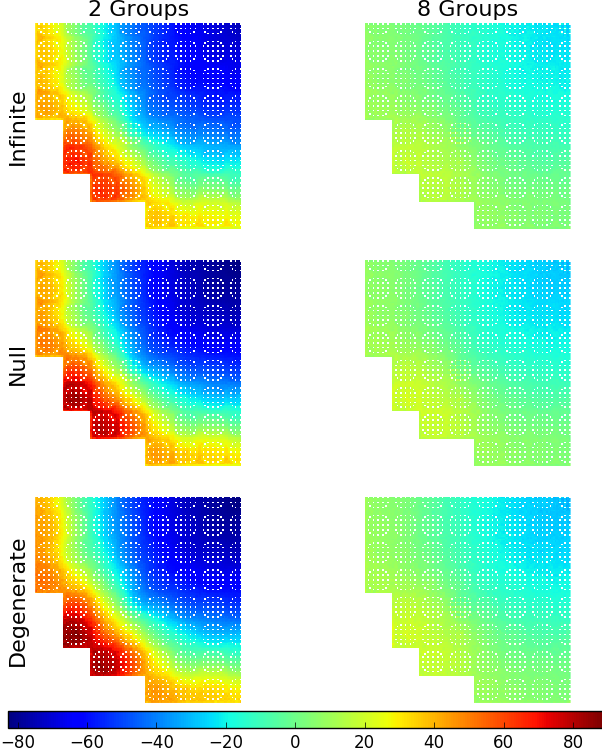
\includegraphics[width=\linewidth]{figures/quantification/appendix/full-core/capt-err}
\vspace{2mm}
\caption[U-238 capture rate errors for the \ac{BEAVRS} quarter core]{U-238 capture percent relative errors rate errors for the 2D quarter core \ac{BEAVRS} model corresponding to the reference in Fig.~\ref{fig:chap7-capt-rates-full-core}.}
\label{fig:quantify-full-core-capt-err}
\end{figure}

\clearpage

%%%%%%%%%%%%%%%%%%%%%%%%%%%%%%%%%%%%%%
\section{Capture Rate Absolute Errors}
\label{sec:quantify-capt-rates-absolute}

The fission and U-238 reaction rates vary much more across pins for benchmarks with leakage due to vacuum boundary conditions, such as the 2$\times$2 colorset and quarter core \ac{BEAVRS} models. In these models, it can be useful to investigate the absolute reaction rate error in addition to the percent relative error (as shown in the preceding sections). The reason for this is that it is important to reduce the error in those pins in which the reaction rates are largest and hence the most limiting to reactor performance (\textit{i.e.}, the hottest fuel pins). The absolute error spatial distributions better illustrate improved reaction rate predictions in the pins that matter most in these benchmark models.

Fig.~\ref{fig:quantify-reflector-capt-err-abs} shows the U-238 capture rate absolute errors between OpenMC and OpenMOC for the null and degenerate spatial homogenizations for 8 and 70 energy groups. Fig.~\ref{fig:quantify-full-core-capt-err-abs} shows the U-238 capture rate absolute errors for the null and degenerate schemes for 40 energy groups. These heatmaps complement the percent relative errors in Figs.~\Crefrange{fig:chap8-reflector-capt-err}{fig:chap8-full-core-capt-err}. The absolute errors are not shown for the four benchmark models with all reflective \acp{BC} since they very closely mirror the percent relative error distributions.

\begin{figure}[h!]
\centering
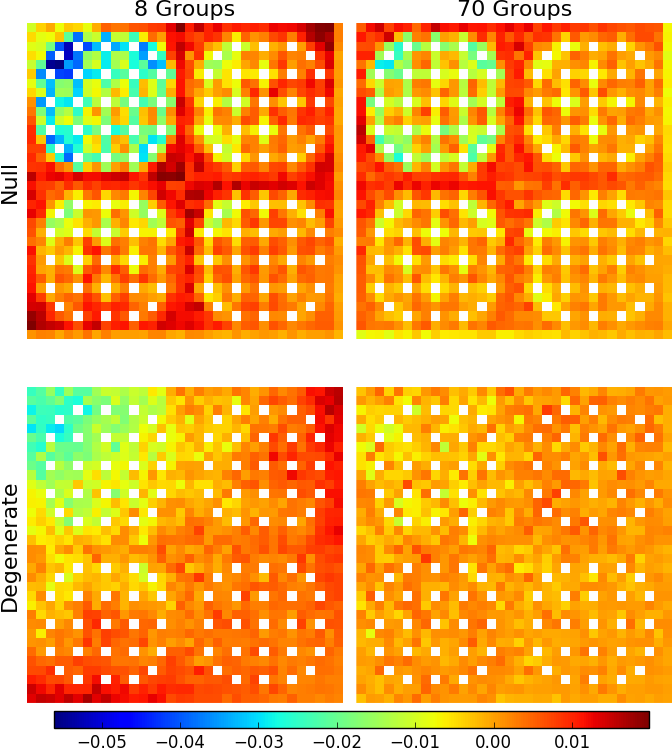
\includegraphics[width=\linewidth]{figures/quantification/appendix/magnitude/reflector/capt-err}
\vspace{2mm}
\caption[U-238 capture rate absolute errors for 2$\times$2 colorset with a reflector]{U-238 capture rate absolute errors for a 2$\times$2 colorset with a reflector corresponding to the reference in Fig.~\ref{fig:chap7-capt-rates-reflector}.}
\label{fig:quantify-reflector-capt-err-abs}
\end{figure}

\clearpage

\begin{figure}[h!]
\centering
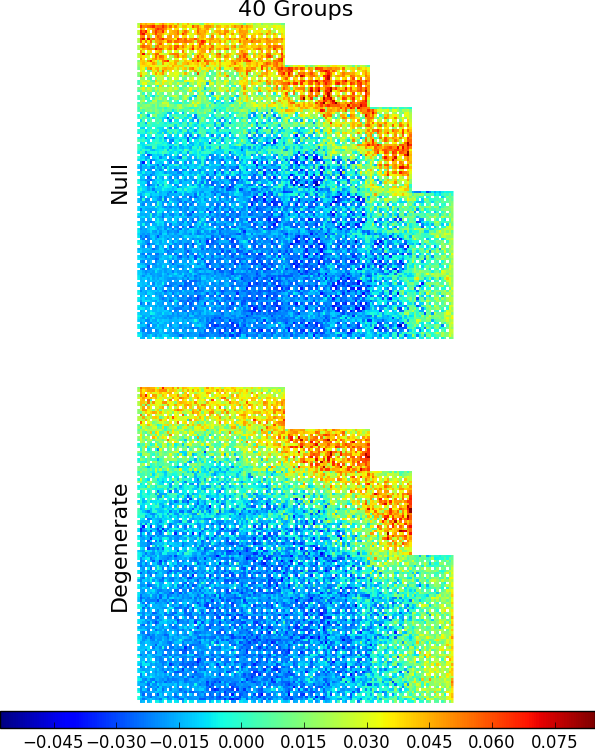
\includegraphics[width=\linewidth]{figures/quantification/appendix/magnitude/full-core/capt-err}
\vspace{2mm}
\caption[U-238 capture rate absolute errors for the \ac{BEAVRS} quarter core]{U-238 capture rate absolute errors for the 2D quarter core \ac{BEAVRS} model corresponding to the reference in Fig.~\ref{fig:chap7-capt-rates-full-core}.}
\label{fig:quantify-full-core-capt-err-abs}
\end{figure}

\clearpage


\end{appendices}
